\chapter{Spécifications}

%Intro\footnotemark\\
%note en bas de page


\section{Environnement}

Notre environnement est une grille carrée de 20 lignes et 20 colonnes donc 400 cellules de type "test\_grid". A partir de chaque cellule, il est possible d'obtenir la liste de ses 4 voisins les plus proches; celui de gauche, celui de droite, celui d'en haut et celui d'en bas. Toutes les interactions se font dans cet environnement.\\

%inclusion d'une mage dans le document
\begin{figure}[!h]
\begin{center}
%taille de l'image en largeur
%remplacer "width" par "height" pour régler la hauteur
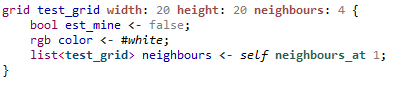
\includegraphics{code/test_grid}
\end{center}
%légende de l'image
\caption{Définition d'une grille de l'environnement}
\end{figure}

%Contenu de la note précédemment marquée avec \footnotemark
%\footnotetext{Note bas de page "intro"}


\section{Minerais}

Pour représenter les minerais dans l'environnement, nous prenons aléatoirement autant de cellules que de minerais que nous voulons représenter. Afin de faire de ces cellules des mines, nous leur attribuons un état miné pour de dire qu'elles contiennent des mines. Aussi, nous colorons les cellules minées en noir.

%inclusion d'une mage dans le document
\begin{figure}[!h]
	\begin{center}
		%taille de l'image en largeur
		%remplacer "width" par "height" pour régler la hauteur
		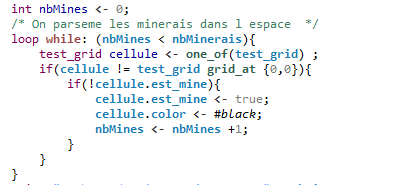
\includegraphics{code/minerais}
	\end{center}
	%légende de l'image
	\caption{Dissémination des minerais}
\end{figure}

\newpage

\section{Base}

Elle représente l’agent passif qu’est la base ici, c’est a dire qu’elle ne fait rien et ne sert ici que de cible de dépôt pour les minerais collectés. Elle sauvegarde la référence vers la cellule de grille dans laquelle elle se trouve. 

\begin{figure}[!h]
	\begin{center}
		%taille de l'image en largeur
		%remplacer "width" par "height" pour régler la hauteur
		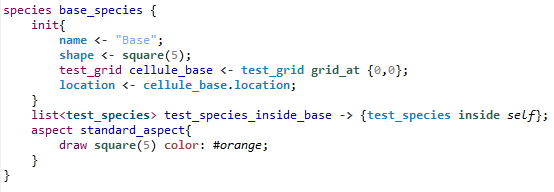
\includegraphics{code/base}
	\end{center}
	%légende de l'image
	\caption{Base de dépôt des minerais}
\end{figure}

\section{Robot réactif}

C’est notre type de robot de base. Il représente des robots réactifs, c’est a dire qui entreprennent des actions qu'en fonction de leur environnement sans aucun apprentissage.  Ils n’ont aucune possibilité de connaitre à l'avance la localisation de la base de dépôt des minerais. Pour trouver la base, ils se déplacent aléatoirement de voisins en voisins jusqu'à’à se trouver à la base Le robot a un nom, sa position actuelle dans l'environnement ainsi que le minerai qu'il porte (potentiellement). Il a aussi un objectif qui peut être soit de chercher des minerais, soit de prendre un minerai, soit d'aller a la base, soit de déposer un minerai a la base.\\
Lorsqu'on l'introduit dans l'environnement lors de l'initialisation, son objectif est de chercher un minerai. Des qu'il en trouve, son objectif devient d'aller a la base. Une fois a la base, il doit y déposer le minerai. Ses objectifs sont atteints à l'aide de réflexes\footnotemark.\\

Dans le cas de notre robot réactif, les réflexes définis sont les suivants:
\begin{itemize}
\item \textbf{chercher\_minerai} qui permet au robot de rechercher des minerais dans l'environnement;
\item \textbf{prendre} qui permet au robot de prendre un minerai trouvé;
\item \textbf{aller\_base} qui permet au robot d'aller à la base;
\item \textbf{deposer} qui permet au robot de déposer un minerai dans la base.
\end{itemize}

\begin{figure}[!h]
	\begin{center}
		%taille de l'image en largeur
		%remplacer "width" par "height" pour régler la hauteur
		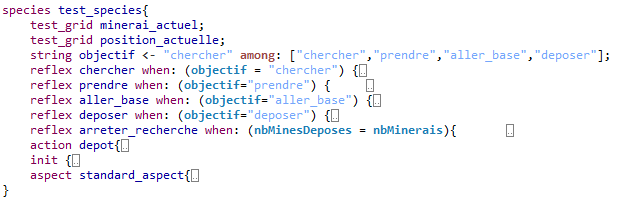
\includegraphics{code/robot_reactif}
	\end{center}
	%légende de l'image
	\caption{Robot réactif}
\end{figure}

\footnotetext{Les réflexes sont des ensembles d'instructions qui s'exécutent après chaque cycle du robot (pas de temps). Elles représentent ainsi les compétences spécifiques des agents et correspondent aux opérations d'une classe ou aux activités dans un diagramme d'activité. }

\section{Robot cognitif }
C’est notre deuxième type de robot. Il s'agit d'une version améliorée du robot réactif. Ce robot a les mêmes réflexes que le premier type de robot. La différence se trouve au niveau du réflexe aller\_base qui est faite ici de façon plus intelligente. En effet, tout comme le robot réactif, le robot cognitif n'a aucune connaisance de l'emplacement de la base à l'avance. Mais, une fois après y être allé, il mémorise cet emplacement. Cela fait qu'après, il ne recherche plus la base mais y va directement en prenant le chemin le plus court.
\begin{figure}[!h]
	\begin{center}
		%taille de l'image en largeur
		%remplacer "width" par "height" pour régler la hauteur
		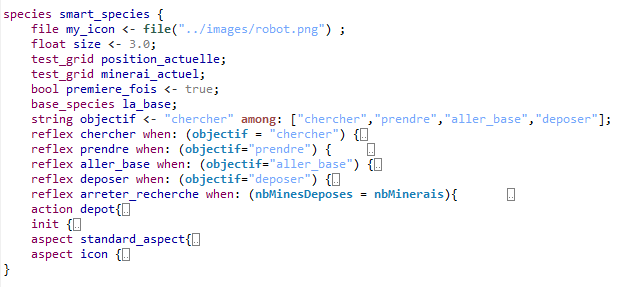
\includegraphics{code/robot_cognitif}
	\end{center}
	%légende de l'image
	\caption{Robot cognitif}
\end{figure}
